
\section{Lunar Coordinate System} \label{sec:lunar} 
As noted in section \ref{sec:gen}, all solar system bodies have their inertial coordinate systems center at the body and are co-aligned with the ICRF system. The body fixed system for the Moon is defined in JEOD as principal axis-based lunar coordinate frame to define the directions of the Moon's rotation pole and prime meridian. The transformation from inertial to fixed are provided by the JPL DE421 Ephemerides. 
The numerically integrated physical librations of the Moon are obtained directly from the DE ephemeris file (JPL recommends DE-421, for lunar orientation). The lunar libration paper \cite{LL} defines three (Euler) angles that describe the orientation of the principal axes of the Moon relative to the ICRF reference frame as follows:   
The three Euler angles are
\begin{itemize}
 \item $\phi$ the angle along the ICRF equator, from the ICRF X-axis to the ascending node of the lunar equator; 
 \item $\theta$ the inclination of the lunar equator to the ICRF equator.
 \item $\psi$ the angle along the lunar equator from the node to the lunar prime meridian
 \end{itemize}
The three Euler angles (or libration angles) are illustrated in Figure \ref{fig:6}.

\textbf{Coordinate Frame: } The body centered body fixed frame.

\begin{itemize}
\item X-axis: Points in the direction of the Moon's prime meridian principal axis (minimum moment of inertia).
\item Y-axis: Completes a standard, right-handed coordinate frame.
\item Z-axis: Points in the direction of the Moon's North pole principal axis (maximum moment of inertia).
\end{itemize}

\begin{figure}[htp]
\centering
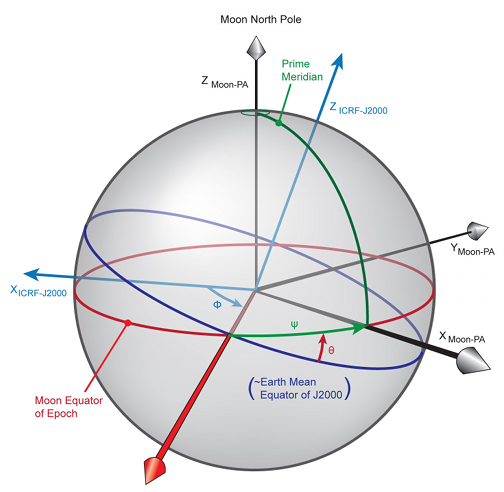
\includegraphics [width=7in]{figs/fig6.png}
\caption{Lunar Inertial and Fixed System}
\label{fig:6}
\end{figure}

\subsection{Example Lunar Coordinate System}
The Moon fixed coordinates are need for computing the non-spherical gravitational accelerations of the Moon.
\begin{verbatim}
An example of setting and recording the Moon's body fixed coordinates can be found in:
\jeod\verif\Integrated_Validation\SIM_Earth_Moon\SET_test\RUN_clem
Set in the input file:
VEH_OBJ.pfix.reference_name     = "Moon";
Recorded in the Log file for the vehicle state:
"#(VEH_OBJ).pfix.state.cart_coords[0-2]";
\end{verbatim}


